% Chapter 1

\chapter{Neural Network Architecture} % Main chapter title

\label{Chapter3} % For referencing the chapter elsewhere, use \ref{Chapter1} 

\lhead{Chapter 3. \emph{Introduction}} % This is for the header on each page - perhaps a shortened title

\section{Introduction} 

Neural Network is heart of OCR system ,the accuracy of OCR system heavily depends on accuracy of Neural
network . 

\section{Multi layer perceptron }

Multi layer perceptron is one of primitive neural network architecture . It contains artificial neurons
(which mimics the behaviour of human neuron) connected as layers as shown in \ref{fig:feed} The neural
network is trained by calculating loss and updating weights of perceptron  with back propagation algorithm 
most common activation function in percptron is Relu.


\begin{figure}[h]
\centering
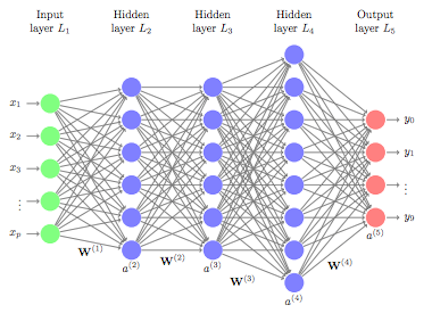
\includegraphics[width=15cm]{Figures/deep_nn.png}
\caption{Multilayer perceptron }
\label{fig:feed}
\end{figure}



\section{Convolutional neural network}
Convolutional Neural Networks  have a structure
similar to MLPs, but each layer is not fully-connected to the previous one. They
implement the notion of local receptors, via local connections and weight sharing. The
input is the two-dimensional image, and neurons in the hidden layers are organized in
two-dimensional maps, each looking for a single feature. Each neuron of a map is only
connected to a small neighborhood in the previous maps (or input image), with the
same connection weights as other neurons of the map . One may interpret
it as convolutions of the image with trainable filters.
\begin{figure}[h]
\centering
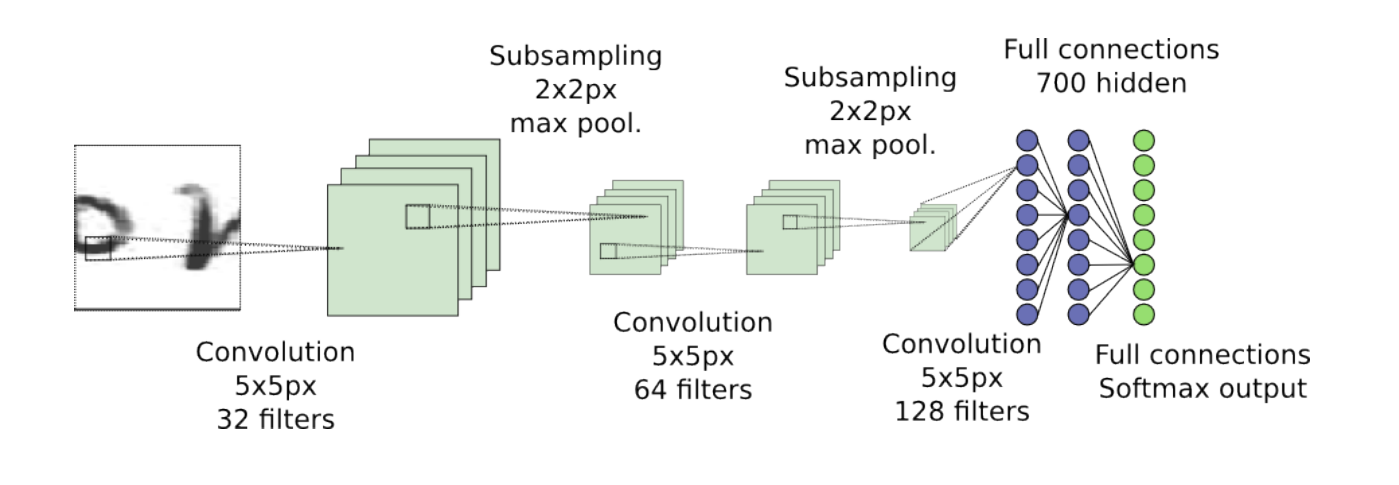
\includegraphics[width=15cm]{Figures/CNN.png}
\caption{ Convolutional neural network}
\label{fig:conv}
\end{figure}

The convolutional layers are often followed by subsampling layers, to limit the size of
the network and implement some invariance to distortions. The subsampling operation
may be a max-pooling or averaging over small neighborhoods. Usually, a few features
(or maps, or trainable filters) are extracted in lower layers, and increasingly more
features are extracted in upper layers, while the dimensions of the maps decrease (e.g.
in LeNet-5 .ConvNNs designed for classification can be easily extended to variable sized images,
hence producing sequences of predictions, thanks to the local connections and shared
weights

\section{Long short-term memory}
The output MLP and CNN just depend on input at present situation but some times we need to depend on the 
previous inputs also. RNN solves this type of problems . In Rnn the present output depends on present input
and also the previous inputs . but Classical RNN suffer from exploding and Vanishing gradient .LSTM Long Short Term Memory solves this issue with forgot gate. 
\begin{figure}[h]
\centering
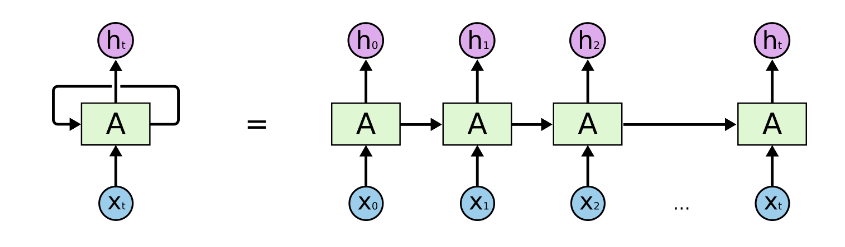
\includegraphics[width=15cm]{Figures/rnn.png}
\caption{ Reccurent neural network}
\label{fig:rnn}
\end{figure}

\begin{figure}[h]
\centering
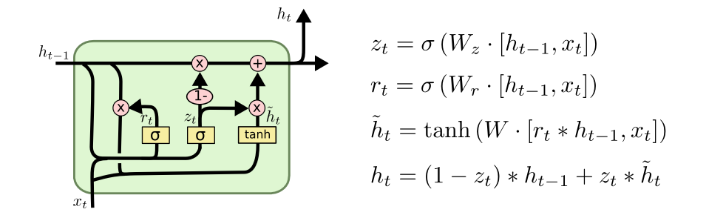
\includegraphics[width=15cm]{Figures/lstm.png}
\caption{ LSTMnetwork}
\label{fig:lstm}
\end{figure}

\section{Connectionist Temporal Classification}
\begin{figure}[h]
\centering
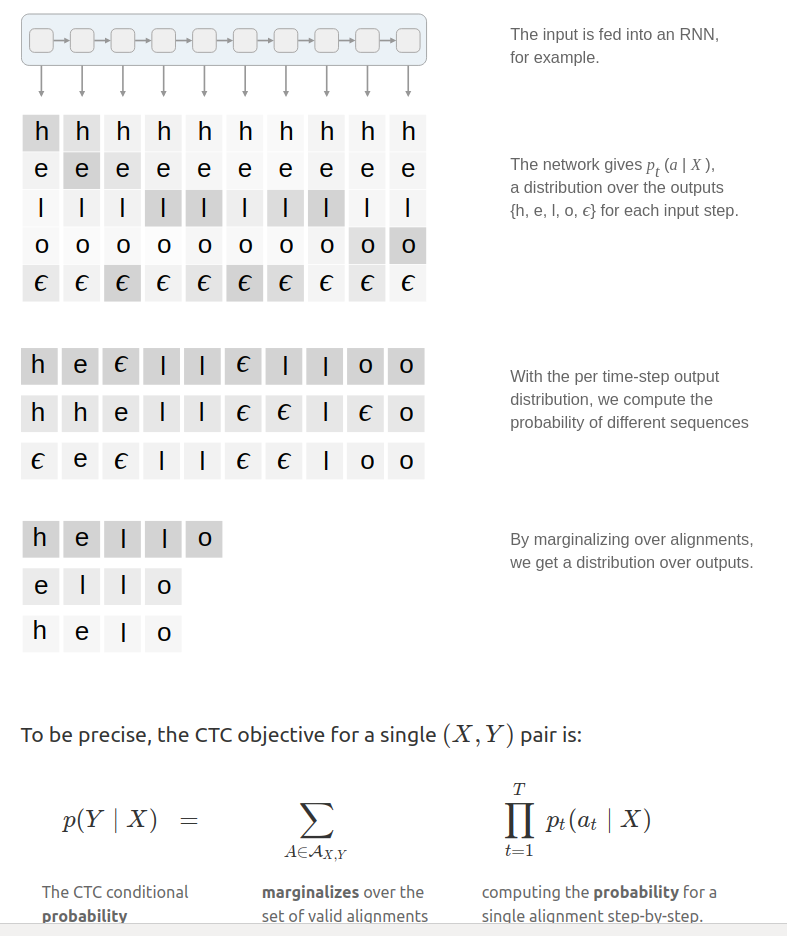
\includegraphics[width=15cm]{Figures/ctc.png}
\caption{ CTC LOSS}
\label{fig:CTC}
\end{figure}


\section{Architecture of OCR Neural Network}

CNN are good at objection recognition and LSTM are good at seq data prediction . To predict the image with
out segmentation we have to feed the image as sequence of pixels.ie we have to predict it with LSTM but LSTM
are hard to train and can't predict well on long sequence. So we have to extract important features from 
image to train a LSTM . CNN comes in handy for extracting  features from given image there by reduces the 
dimension of input. 


The architecture is shown in figure \ref{fig:arch}.The Neural network consist It consists of 7
convolutional layers these layers help to extract the important features to feed to LSTM. 7 CNN layers were
chosen so that the Neural Network will not over fit on large dataset .Batch normalization and drop out
techniques were used to improve the generalization of the network. Finally the Bidirectional LSTM recognizes
the word .Since LSTM are hard to train for long duration the number of CNN layers were kept more to increase
the recognition capacity of the network.CTC loss is used to calculation the loss and train the network
.Language model corrects the CTC decoded output.

\begin{figure}[h]
\centering
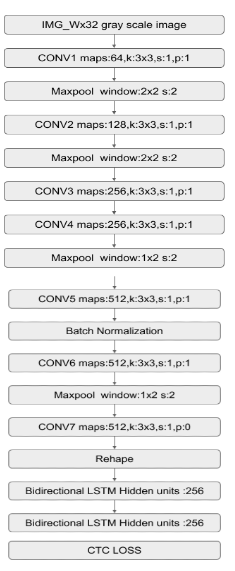
\includegraphics{Figures/arch.png}
\caption{Neural Network Architecture}
\label{fig:arch}
\end{figure}
